Ce présent document s’applique à l’ensemble des livrables conçus dans le cadre du projet, c’est-à-dire à l’ensemble de la documentation produite par les membres de l’équipe. Ces derniers doivent donc prendre connaissance du présent document, tandis que son application se doit d’être contrôlée par le responsable qualité. Lorsque le plan d’assurance qualité est amené à être modifié pour les raisons évoquées dans les paragraphes précédents, le responsable qualité a pour charge de communiquer à l’équipe les changements apportés, afin de veiller à ce que tous les membres soient au fait des nouvelles pratiques à appliquer. \\

Ainsi, tout document produit au sein de ce projet est soumis au procédé ci-dessous, consistant à appliquer le plan d’assurance qualité afin de produire un premier document par la maîtrise d’ouvrage. Le responsable qualité peut alors être amené à réaliser un rappel de ce plan d’assurance qualité auprès de la maîtrise d’ouvrage si certains concepts, procédés ou contraintes n’ont pas été respectés, afin d’obtenir un document normalisé pouvant être soumis à validation. Ce déroulement s’inscrit dans un cycle de vie des documents plus vaste et décrit dans la partie suivante.

\begin{figure}[H]
    \centering
    \label{fig-objec}
    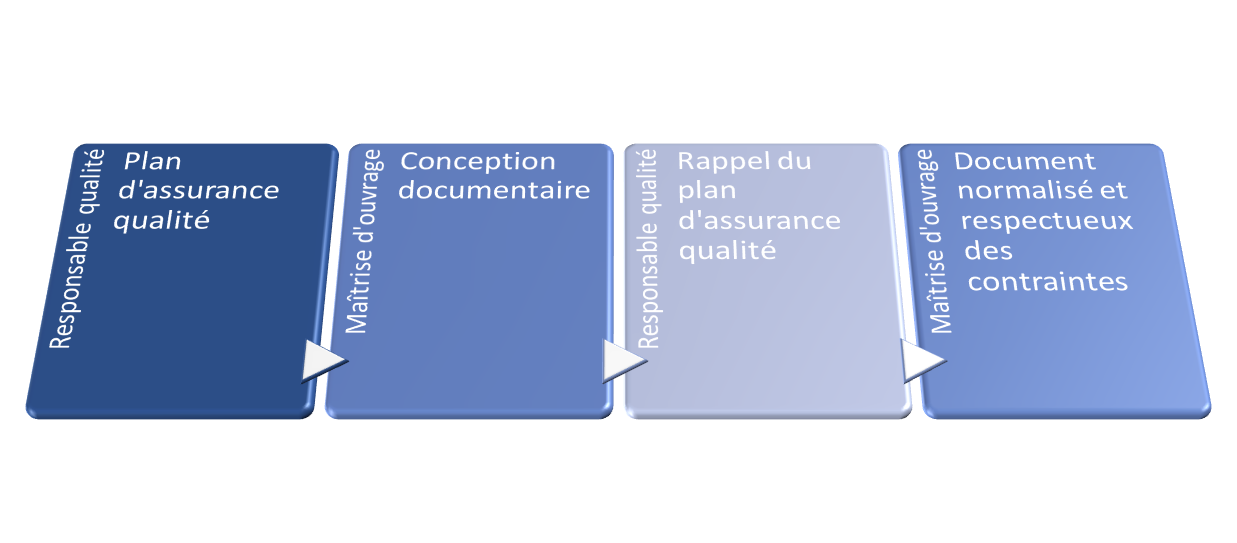
\includegraphics[scale=0.5]{figures/applic_paq.png}
    \caption{Application du plan d’assurance qualité lors de la conception d’un document}
\end{figure}